\newpage
\section{Theoretical Analysis}
\label{sec:analysis}

\subsection{Ideal Operational Amplifier}

The transfer function of the circuit was calculated using an ideal OpAmp, equation \ref{eq:tf}. Through out this function, the module (Figure \ref{fig:idealbode_db}) and phase (Figure \ref{fig:idealbode_f}) of the transfer function was obtained.

\begin{equation}
    T(s)=\frac{R_1C_{eq}s}{1+R_1C_{eq}s}*\left ( 1+\frac{R_3}{R_4} \right )
    \label{eq:tf}
\end{equation}

\begin{figure}[h]
  \centering
  \begin{minipage}[b]{0.45\textwidth}
    \includegraphics[width=1\textwidth]{idealbode_db.eps}
    \caption{Module of the transfer function in frequency response - ideal OpAmp.}
    \label{fig:idealbode_db}
  \end{minipage}
  \hfill
  \begin{minipage}[b]{0.45\textwidth}
    \includegraphics[width=1\textwidth]{idealbode_f.eps}
    \caption{Phase of the transfer function in frequency response - ideal OpAmp.}
    \label{fig:idealbode_f}
  \end{minipage}
\end{figure}

\subsection{Non-Ideal Operational Amplifier}

The process to obtain the transfer function of the circuit for an non-ideal OpAmp, the same process of the ideal OpAmp was used, but the transfer function of equation \ref{eq:tf} was multiplied with the one obtained in section \ref{sec:simulation}, equation \ref{eq:tfsim}, and with an adjust in the gain.

\begin{equation}
    T(s)=\frac{R_1C_{eq}s}{1+R_1C_{eq}s}*\left ( 1+\frac{R_3}{R_4} \right )* \frac{1*10^{10}}{(s+1*10^4)(s+1*10^6)}
    \label{eq:tf+tfsim}
\end{equation}

\begin{figure}[h]
  \centering
  \begin{minipage}[b]{0.45\textwidth}
    \includegraphics[width=1\textwidth]{non_idealbode_db.eps}
    \caption{Module of the transfer function in frequency response - non-ideal OpAmp.}
    \label{fig:nonidealbode_db}
  \end{minipage}
  \hfill
  \begin{minipage}[b]{0.45\textwidth}
    \includegraphics[width=1\textwidth]{non_idealbode_f.eps}
    \caption{Phase of the transfer function in frequency response - non-ideal OpAmp.}
    \label{fig:nonidealbode_f}
  \end{minipage}
\end{figure}

%For theoretical analysis, in a first stage, an ideal OpAmp was used. This 

It was possible to conclude that graphics showed an high pass filter. 

To simulate a pass band filter is necessary to have components that do not allow low and high frequencies to pass. In this case, it was not necessary to use more components to limit the high frequency because the OpAmp was non ideal so simulate a low pass filter.

\newpage
\section{Results Analysis}
\label{sec:resultsanalysis}

In the presented section, the main goal is to compare side by side the results obtained in the simulation with \textit{Ngspice} and the theoretical analysis obtained with \textit{Octave}. Two comparisons will be made. One for the phase and other for the gain of the circuit analysed. 

The following figures (\ref{fig:gfr1} and \ref{fig:nonidealbode_db1}) compare the module of the transfer function in frequency response:

\begin{figure}[h]
  \centering
  \begin{minipage}[b]{0.45\textwidth}
    \includegraphics[width=1\textwidth]{Vo1db.pdf}
    \caption{Gain in Frequency Response.}
    \label{fig:gfr1}
  \end{minipage}
  \hfill
  \begin{minipage}[b]{0.5\textwidth}
    \includegraphics[width=1\textwidth]{non_idealbode_db.eps}
    \caption{Module of the transfer function in frequency response - non-ideal OpAmp.}
    \label{fig:nonidealbode_db1}
  \end{minipage}
\end{figure}

Analysing the two images \ref{fig:gfr1} and \ref{fig:nonidealbode_db1}, it is possible to observe that they are very similar because, in the theoretical analysis, it was considered a non-ideal OpAmp as well as in simulation with \textit{Ngspice}. The same can be seen in figures \ref{fig:pfr1} and \ref{fig:nonidealbode_f1} that compare the phase in both cases.

\begin{figure}[h]
  \centering
  \begin{minipage}[b]{0.45\textwidth}
    \includegraphics[width=1\textwidth]{Vo1f.pdf}
    \caption{Phase in Frequency Response.}
    \label{fig:pfr1}
  \end{minipage}
  \hfill
  \begin{minipage}[b]{0.5\textwidth}
    \includegraphics[width=1\textwidth]{non_idealbode_f.eps}
    \caption{Phase of the transfer function in frequency response - non-ideal OpAmp.}
    \label{fig:nonidealbode_f1}
  \end{minipage}
\end{figure}
\newpage
The value found for the merit is calculated with the following expression (equation \ref{eq:merit}):

\begin{equation}
    M= \frac{1}{Cost\ast (Voltage \, Gain \, Deviation + Central\, Frequency\, Deviation+10^{-6})}
  \label{eq:merit}
\end{equation}

In the equation \ref{eq:merit}, the voltage gain deviation is the difference between the required value for the gain (100 or 40dB) and the value obtained (99.87576 or 39.98920dB). Taking this into account, the value for the voltage gain deviation used in the merit equation is 0.12424 (100-99.87576).    

In order to find the central frequency deviation, a constant line in minus 3dB from the maximum value was drawn. The intersection between this line and the graph gives two values for the frequency- low and high. The low frequency corresponds to the lower value and the high frequency to the higher value of the frequency. The following image explains these procedure (image \ref{fig:central_frequency_deviation}):

\begin{figure}[h] \centering
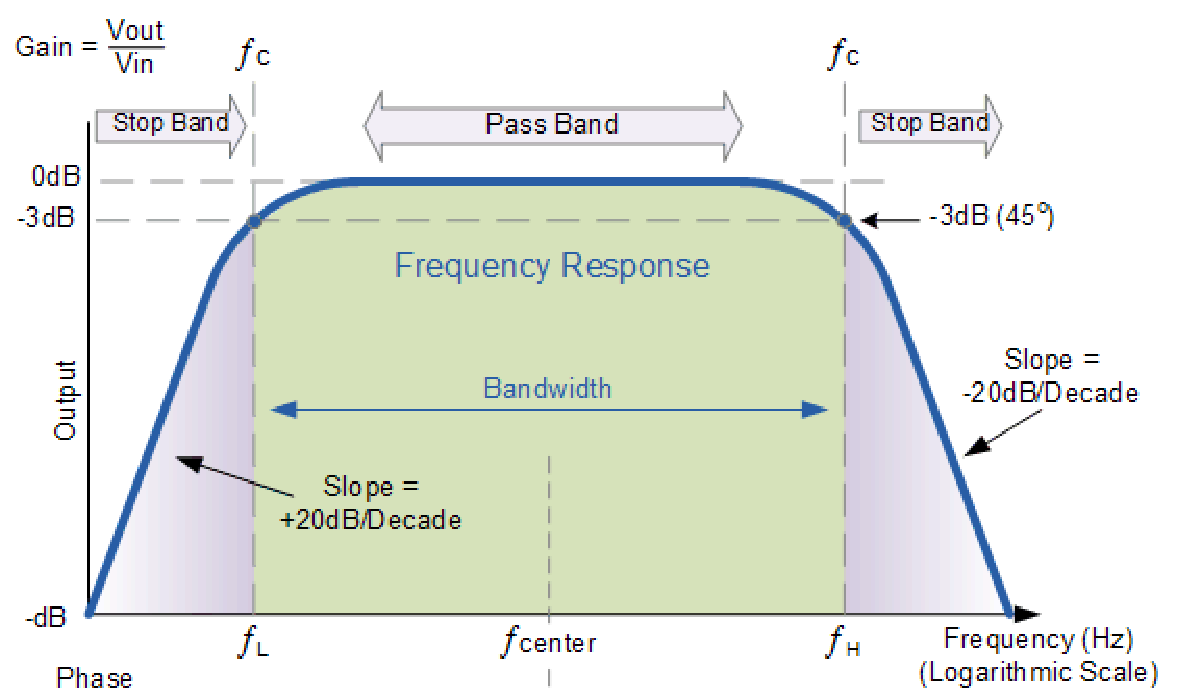
\includegraphics[width=0.7\linewidth]{central frequency deviation.pdf}
\caption{Calculation of the central frequency deviation}
\label{fig:central_frequency_deviation}
\end{figure}

\newpage
\begin{equation}
    frequency\:deviation =\left | 1000 - \sqrt{f_{low} \times  f_{high}} \right |=\left | 1000 - \sqrt{105.0228 \times 10117.16} \right |=30.79215715
    \label{eq:freq}
\end{equation}


The cost was calculated based on the components used. For design this circuit were used 5 diodes, 2 transistors, 12 resistances and 5 capacitors. The total cost is 13428.29504 MU.

Using equation \ref{eq:merit} and the values of each variable described above, the merit using the formula at \ref{eq:merit}, is:

\begin{equation}
    M = 2.408741713 * 10^{-6}
    \label{eq:meritf}
\end{equation}


















